\chapter{Resultados}\label{chapter: Results}
%Experimentación 

En este capítulo se presentan variantes de problemas de enrutamiento de vehículos a los que no era posible aplicarle la evaluación automática sin realizar modificaciones en el código. Se presentan los cambios necesarios para aplicar la evaluación automática a estos problemas.

Este capítulo se divide en 3 secciones. La sección \ref{4:VRPSPD} presenta la evaluación de vecinos del Problema de Enrutamiento de Vehículos con Recogidas y Entregas. La sección \ref{4:VRPTW} presenta la evaluación de vecinos del Problema de Enrutamiento de Vehículos con Ventanas de Tiempo. La sección \ref{4:Ext} presenta la extensibilidad de este trabajo.

\section{VRP con Recogidas y Entregas simultáneas}\label{4:VRPSPD}
En esta sección se aplica la evaluación automática a un problema de enrutamiento de vehículos con Recogidas y Entregas simultáneas (VRPSPD). Este problema se explica en el capítulo \ref{chapter: Automatic-Eval}, en la sección \ref{3:VRP-limits}.

La figura \ref{fig:VRPSPD-init} muestra una solución inicial de un VRPSPD. Este ejemplo presenta dos rutas, con vehículos de capacidad 20 y 15 respectivamente. El primer vehículo sale del depósito con 5 productos y vista los clientes 1, 2 y 3. El segundo vehículo sale del depósito sin productos y visita los clientes 4 y 5. Cada cliente entrega y recibe un cantidad de productos una vez que es visitado. La cantidad que entrega y que recibe se observa en el nodo que representa a cada cliente.

\begin{figure}[htb]
	\centering
	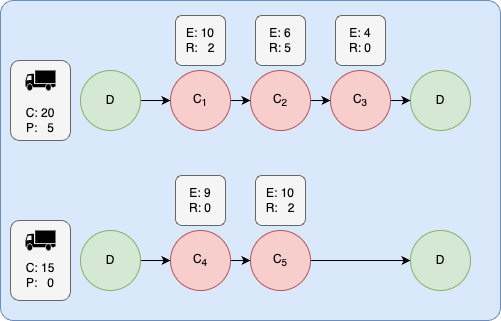
\includegraphics[width=0.5\linewidth]{Graphics/VRPSPD}
	\caption{ Solución inicial del VRPSPD.}
	\label{fig:VRPSPD-init}
\end{figure}

Se deben satisfacer las demandas de cada cliente y obtener la menor distancia para las rutas. El pseudocódigo de la evaluación de la solución inicial se presenta en la figura \ref{vrpspd-sol-code}.

\begin{figure}[h!]
    \begin{verbatim} 
  1  evalúa(S):
  2    new_var distancia_total = 0
  3    para toda ruta r de S:         
  4        new_var demanda_ruta = 0
           new_var penalización = 0
  5        new_var cliente_previo = deposito(r)
  6        para todo cliente c en r:
  7            incrementa distancia_total con...
                          d(cliente_previo, c)
  8            incrementa demanda_ruta con demandas de c 
  9            si demanda_ruta > capacidad del vehículo...
                                 de la ruta r:
  10                penalizar_en_cinta(c)
                    incrementar penalización( 
                        demanda_ruta - capacidad...
                        del vehículo de la ruta r)
  11           cliente_previo = c
  12       incrementa distancia_total con...
                d(c, depósito) 
  13       incrementa distancia_total con penalización
  14    devuelve distancia_total        
  \end{verbatim}
    \caption{Código de evaluación de una solución de un VRPSPD. La operación \texttt{d(x,y)} representa la distancia entre \texttt{x} e \texttt{y}.\label{vrpspd-sol-code}}
\end{figure}

Las demandas del cliente en este problema son los productos que entrega el cliente menos los productos que recoge.

La función $penalizar\_en\_cinta$ guarda el cliente c en la cinta automática en caso de que la demanda de la ruta exceda la capacidad del vehículo en el momento en que se visita al cliente c. Al aplicar los criterios de vecindad en la solución se debe comprobar en la cinta los clientes que penalizaron las rutas antes de evaluar la nueva solución.

 \section{VRP con Ventanas de Tiempo}\label{4:VRPTW}
 En esta sección se aplica la evaluación automática a un problema de enrutamiento de vehículos con Ventanas de Tiempo (VRPTW). Este problema se explica en el capítulo \ref{chapter: Automatic-Eval}, en la sección \ref{3:VRP-limits}.
 
 La figura \ref{fig:VRPSPD-init} muestra una solución inicial de un VRPTW. Este ejemplo, igual que el anterior presenta dos ruta. Cada cliente tiene una hora mínima y una hora máxima entre las que puede ser recogido. Si el vehículo no llega entre esas horas significaría una penalización en la ruta.
 
 \begin{figure}[htb]
     \centering
     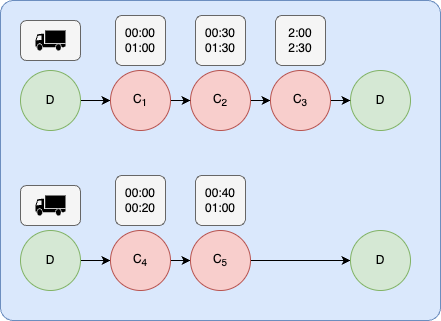
\includegraphics[width=0.5\linewidth]{Graphics/VRPTW}
     \caption{ Solución inicial del VRPTW.}
     \label{fig:VRPSPD-init}
 \end{figure}
 
El pseudocódigo de la evaluación de la solución inicial se presenta en la figura \ref{vrptw-sol-code}.
 
 \begin{figure}[h!]
     \begin{verbatim} 
   1  evalúa(S):
   2    new_var distancia_total = 0
   3    para toda ruta r de S:         
   4        new_var tiempo_ruta = 0
            new_var penalización = 0
   5        new_var cliente_previo = deposito(r)
   6        para todo cliente c en r:
   7            incrementa distancia_total con...
                           d(cliente_previo, c) 
                incrementa tiempo_ruta con...
                           t(cliente_previo, c)
   9            si tiempo_ruta < tiempo mínimo de c
   10                penalizar_en_cinta(c)
                     incrementa penalización con...
                        tiempo_ruta - tiempo mínimo de c
                si tiempo_ruta > tiempo máximo de c
   11                penalizar_en_cinta(c)
                     incrementa penalización con...
                        tiempo máximo de c - tiempo_ruta

   12           cliente_previo = c
   13       incrementa distancia_total con...
                 d(c, depósito)
            incrementa tiempo_ruta con...
                 t(c, depósito) 
   14       incrementa distancia_total con penalización
   15    devuelve distancia_total        
   \end{verbatim}
     \caption{Código de evaluación de una solución de un VRPTW. La operación \texttt{d(x,y)} representa la distancia entre \texttt{x} e \texttt{y}. La operación \texttt{t(x,y)} representa el tiempo del recorrido entre \texttt{x} e \texttt{y}\label{vrptw-sol-code}}
 \end{figure}

La cinta de evaluación automática guarda los clientes que no fueron recogidos en los tiempos asignados. Al aplicar los diferentes criterios de vecindad para modificar la solución y encontrar vecinos se tienen en cuenta las penalizaciones de los clientes para evaluar toda la ruta o a partir del cliente que se modifica. De esta manera se pueden encontrar soluciones vecinas y evaluarse de manera automática, no solo en estos problemas sino en cualquier VRP, que es el objetivo de este trabajo.

En la siguiente sección se presenta cómo extender la propuesta a otros problemas de enrutamiento de vehículos.

\section{Extensibilidad}\label{4:Ext}

En esta sección se comentan algunos problemas diferentes a los presentados en la sección anterior y que se le puede aplicar la evaluación automática.

Para cada variante de VRP deben implementarse diferentes operaciones, no solo mover clientes. Por ejemplo, en el Problema de Enrutamiento de Vehículos con Múltiples Depósitos (MDVRP) se tiene una lista de depósitos y las rutas pueden iniciar y terminar en depósitos distintos. Por ese motivo es necesario implementar las operaciones cambiar el primer depósito de una ruta y cambiar el último depósito de una ruta. Estas operaciones pueden realizarse de la misma manera que las inserciones y extracciones de clientes y el nuevo depósito a insertar se toma de la lista de depósitos disponibles.

Las operaciones implementadas se usan en la cinta computacional para evaluar las soluciones vecinas de la misma manera que se expuso en este capítulo.

A continuación se presentan las conclusiones y recomendaciones del presente trabajo.
% Conclusiones, recomendaciones y bibliografía





























